\chapter{Jumping Right In, TLDR sytle}
If you're the kind of haxor that doesn't want to read a huge book and just wants to get hacking ASAP, this chapter is for you!! This chapter will make a few assumptions. Firstly, it is assumed that you are in a linux environment and will have command of the line that takes commands. Coincidental, this is commonly referred to as the \emph{command line}. Secondly, this command line will be one that accepts linux style commands in a \texttt{bash} format. If you've never heard of bash, Google it. Thirdly and lastly, you will be using the only IDE true ninjas use, namely \texttt{VSCode}. If these conditions apply to your environment, you're good. If they don't but you use Linux, you're still good (as you're almost certainly competent enough at this stuff to be able to easily be able to make the necessary adjustments to get things working in your environment.)

We start this journey from the perspective of having a fresh vanilla install of the minimal version of Ubuntu 20+. Ubuntu is a distribution or (flavor) of linux that is likely the most popular and accessible in the market. I say likely because I don't know for sure, but if it isn't I'd be shocked!

\section{Installation}
First and foremost, lets check what os we're running at the moment.
\par
\shellout{tldr_checkos.shell}
Ok good, we're running Ubuntu 20.04.4 LTS as the \texttt{PRETTY\_NAME=} indicates.

Now immediately execute \texttt{sudo apt update} and \texttt{sudo apt upgrade} as two separate commands, don't ask why just do it.

\subsection{Python Environment}
\par
Next, we need to have Python installed. Python is the programming language and runtime that Jaseci is primarily built upon. It's also the language that 99.999\% of everyone uses for AI research and products (and myriad other things). It's also my favorite as of late, well, second favorite after Jac. Lets check to see. Simply enter the command,
\par
\shellout{tldr_checkpython.shell}
Some of you at this point might see a python version that is >= 3.8. If you see this you're good, you have Python installed. We don't see this in this example. That is because we have the \emph{minimal} Ubuntu. So we have to install it.
\par
\shellout{tldr_installpython.shell}
\par
The line \texttt{sudo apt install python3 python3-pip} instructs Ubuntu to install both the \texttt{python3} package as well as the \texttt{python3-pip} package. Note in the example there is a point where it will ask you if you want to continue, just press Y and let it go. This step could take some time in principle, but we are almost there!

\par
Lets next check again that we have python installed.
\par
\shellout{tldr_checkpython2.shell}

Yes! We're in great shape, we've also checked that \texttt{pip} is install and that looks good as well. Note that we can also replace \texttt{pip} with \texttt{pip3} and everything should work as well.

\subsection{Installing Jaseci}

Now that we have Python setup, we can use the \texttt{pip} install Jaseci itself. \texttt{pip} is Python's official package manager. This command line tool allows users of Python to install packages or code libraries that go beyond the standard libraries that come with Python out of the box. There is a public repository of libraries that is open to all the haxors of the world called PyPI~\cite{PyPI} that houses pretty much all the published python packages of the world. Jaseci lives there throuh two packages, \texttt{jaseci} and \texttt{jaseci-serv}. For the moment we need only concern ourselves with \texttt{jaseci} as we get started. When we're ready to launch amazing tech stacks to production on scalable cloud infrastructure we'll pull down \texttt{jaseci-serv}.

Now, lets install Jaseci!
\par
\shellout{tldr_jsinstall.shell}

TADA! We've pulled down Jaseci and are good to go! In this case we've installed Jaseci version \texttt{1.3.1.1}, your version should be at least this one but probably higher depending on when you're reading this. If its say a year after this moment that I'm writing this book and it's still 1.3.1.1, something very very wrong has happened. Indeed, if its two weeks later and nothing has changed, call 911 and report a missing person, seriously.

To validate that everything works, lets check the command line tool \texttt{jsctl} is present. \texttt{jsctl} is a command line tool that give full control and access to the Jaseci computational model. In particular, and for the sake of this chapter, we will use this tool to build and run programs, generate source for visualizing data and graphs, building artificial intelligence (AI) programs, hot loading fancy AI models, pushing implementations live to Jaseci servers and much much more. Now lets make sure we have access to this very powerful cli tool.

\par
\shellout{tldr_jsctlhelp.shell}

If you see this output, you're in business!! If you don't, something went wrong and you should phone a friend, (but first make sure you didn't miss anything above).

\subsection{VSCode and the Jac Language Extension}

This is technically optional but... I strongly recommend you install and use VSCode with Jaseci. VSCode \gls{IMHO}, is the best code editor on the planet. I regard it as the choice Sake to sip with my Jaseci omakase. Personally, I use an Ubuntu flavored \gls{WSL} VSCode environment.

\begin{figure}
    \centering
    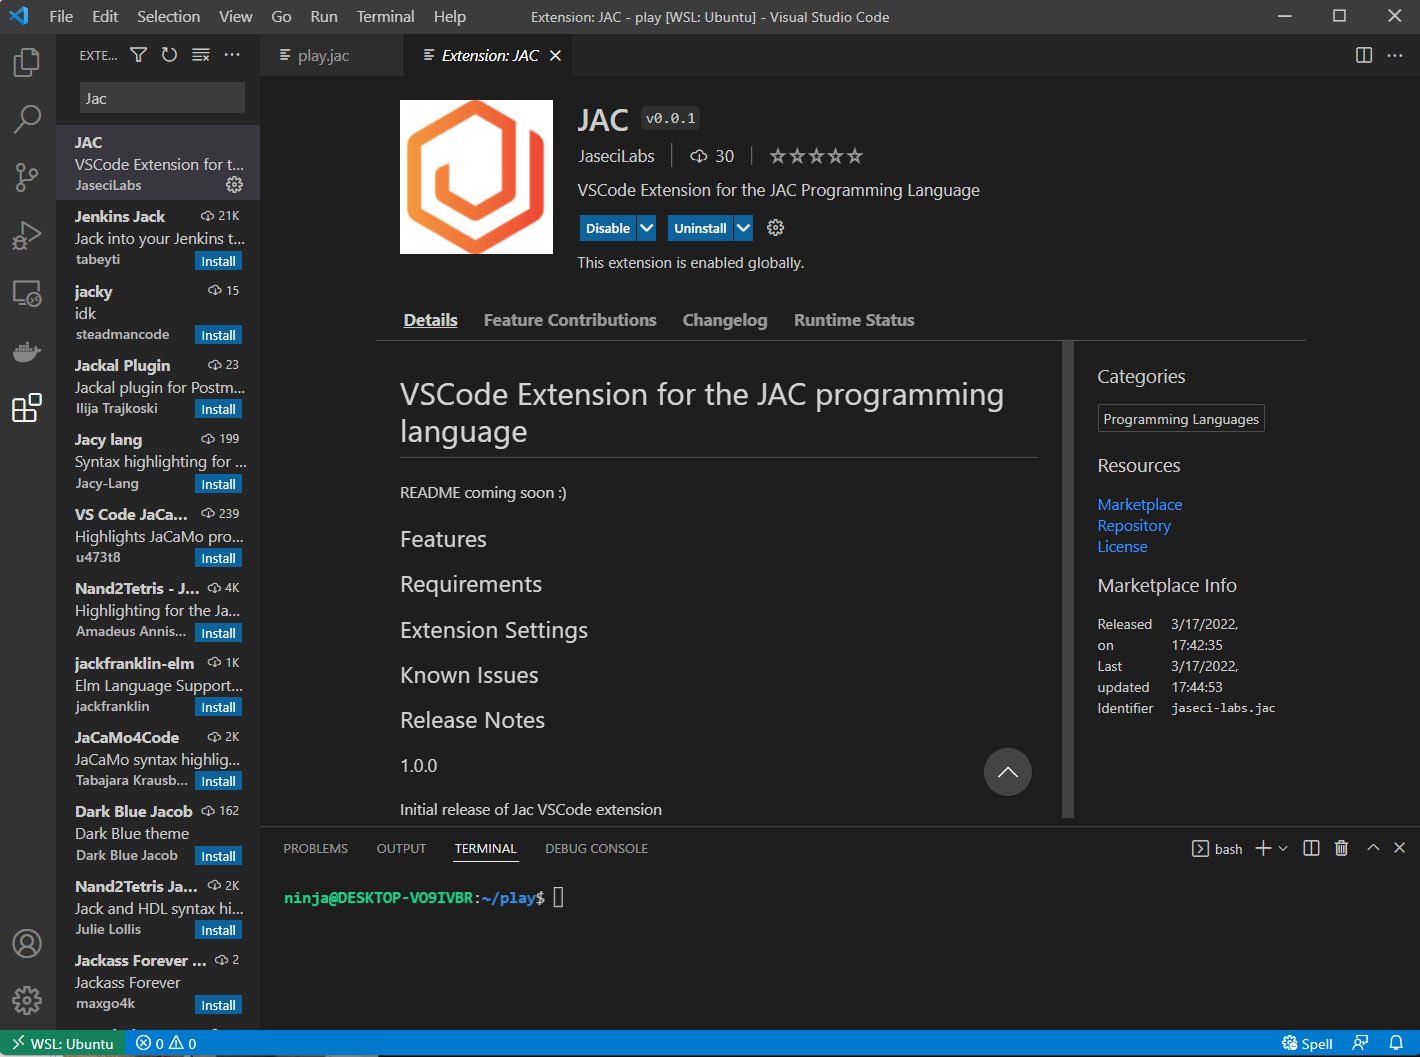
\includegraphics[width=.7\linewidth]{assets/images/vscode_jac_plugin.png}
    \caption[]{The Wonderful Jac Language extension in VSCode.}
    \label{fig:vscode_jac}
\end{figure}

\par
In VSCode, you can search for and install the Jac language extensions as per Figure~\ref{fig:vscode_jac}. As you can see, at the time I clipped this image, its quite new and doesn't really have a readme. You won't need one, it just provides syntax highlighting for \texttt{.jac} files at the moment. But it makes Jac code look beautiful, so it's a must have.

\section{Coding in Jac}

Jac, which is short hand for \textbf{Ja}seci \textbf{C}ode,  is a programming language designed for building programs for Jaseci. The language itself is inspired by a mixture of Javascript and Python and can be used standalone or as glue code for libraries built in other languages ecosystems. Jac is to Python, what Python is to C, what C is to assembly language for scalable sophisticated applications running in the cloud. In this section, we'll cover basics to advanced assuming no programming experience. Though we'll try to cover everything from first time coders to pros, we'll move fast through some of the rudimentary concepts so have your Google ready if you need to drill in a bit more of some of the basic programming concepts. Lets Jump in!

\subsection{Jac Basics}

Launch VSCode, spool up a terminal window, and lets tinker with an example. We'll start with Jac Code~\ref{jac:tldr_hello.jac}. I'd strongly recommend you type out this example (instead of cutting and pasting) especially if this might be your first time programming or are a little rusty with Python and or Javascript. It's the best way to learn!

\par
\jaccode{tldr_hello.jac}{Example program introducing basic syntax.}

This first example Jac Code~\ref{jac:tldr_hello.jac} shows a simple program example demonstrating a number of basic language features. Firstly, observe that the first three assignments in the program to \texttt{x}, \texttt{y}, and \texttt{z} does not specify any types indicating that Jac is a \gls{dynamically typed language}. This means the types are inferred from the assignment of variables, and these types can change dynamically as new assignments are applied to the same variables. This feature is designed to work almost exactly like the dynamic typing in Python.

\par
Next we find a conditional statement much like any other language. Do note operators like the Python inspired \lstinline{or} is supported along side the C/C++/Javascript \lstinline{||} operator. Other such operators include \lstinline{and} (\lstinline{\&\&}), \lstinline{not} (\lstinline{!}), etc.

\par
After the conditional we have a library call \lstinline{std.out(x)} on line 11. This call prints the value of x to the screen. \lstinline{std.out} in Jac is equivalent to the the \texttt{print} in Python and analogous to the \texttt{printf}, \texttt{cout}, and \texttt{console.log} you'd find in C, C++, and Javascript respectively. A suite of core standard library operations for the language has the preamble of \lstinline{std}.

Output:
\shellout{tldr_hello.jac.output}


\subsection{Types in Jac}
[Types example]
\jaccode{tldr_types.jac}{First Example}
Output:
\shellout{tldr_types.jac.output}

\subsection{Fun with Lists and Dictionaries}
[Fun with Lists and Dictionaries]
\jaccode{tldr_listdict.jac}{First Example}
Output:
\shellout{tldr_listdict.jac.output}

\subsection{Control Flow}
[Fun with Control Flow]
\jaccode{tldr_control.jac}{First Example}
Output:
\shellout{tldr_control.jac.output}

\subsection{Graphs in Jac}
[Bringing Graphs in with special operators]
\jaccode{tldr_graph.jac}{First Example}
\jacdotnw{tldr_graph}{.7}{Graph in memory for JC~\ref{jac:tldr_graph.jac}}
Output:
\shellout{tldr_graph.jac.output}

\subsection{Navigating Graphs with Walkers}
[Walking Graphs]
\jaccode{tldr_graphwalk.jac}{First Example}
\jacdotnw{tldr_graphwalk}{.7}{Graph in memory for JC~\ref{jac:tldr_graphwalk.jac}}
Output:
\shellout{tldr_graphwalk.jac.output}

\subsection{Compute in Nodes}
[Compute into the Nodes]
\jaccode{tldr_nodecompute.jac}{First Example}
\jacdotnw{tldr_nodecompute}{.4}{Graph in memory for JC~\ref{jac:tldr_nodecompute.jac}}
Output:
\shellout{tldr_nodecompute.jac.output}

\subsection{Static Graphs}
[Static graphs]
\jaccode{tldr_staticgraph.jac}{First Example}
\jacdotnw{tldr_staticgraph}{.97}{Graph in memory for JC~\ref{jac:tldr_staticgraph.jac}}

\subsection{Writing Tests}
[Tests]
\jaccode{tldr_test.jac}{First Example}
Output:
\shellout{tldr_test.jac.output}

\section{Jac Hacking Workflow}
In this section, we discuss a typical workflow and organization of a Jac coding project. To this end, we will be creating a simple toy chatbot project and examine it's file organization and development workflow. First, lets take a look at the files for this project.
\par
\shellout{tldr_wf_ls.shell}

Now lets take a look a what each of these files represent:

\begin{itemize}
    \item \texttt{cai.jac} - This is the main file for the project to which the various other elements (nodes, edges, graphs, etc) are imported from other files in the directory.
    \item \texttt{nodes.jac} - This file houses the node architypes created for this application. Functionality is specified in both the walkers and as node abilities.
    \item \texttt{edges.jac} - This file contains the edge architypes we've specified in the design of our conversational AI. These edges represent various types of transitions we can make throughout the converstation.
    \item \texttt{static\_conv.jac} - This file contains a static conversational graph that represents the posible conversational flows via state nodes and transition edges.
    \item \texttt{load\_faq.jac} - This file contains a static constructor for graph elements to correspond to frequently asked questions by loading them from a file.
    \item \texttt{faq\_answers.txt} - This file specifies a list of answers to frequently asked questions, we'll be using a model that only depends on the answers themselves.
    \item \texttt{tests.jac} - This file is where we house all the tests for our project.
\end{itemize}

\subsection{Using Imports}

\jaccode{tldr_wf_cai.jac}{Main CAI Jac App}

\jaccode{tldr_wf_nodes.jac}{Nodes for CAI}

\jaccode{tldr_wf_edges.jac}{edges for CAI}

\subsection{Leveraging Static Graphs for Quick Prototyping}
\jaccode{tldr_wf_static_conv.jac}{Static Conversational Graph}

\subsection{Test Driven Development}
\jaccode{tldr_wf_tests.jac}{Tests for CAI}

\subsection{File I/O}
\jaccode{tldr_wf_load_faq.jac}{FAQ Graph Loader}
\shellout{tldr_wf_faq_answers.txt}


\subsection{Building to JIR}

\section{AI with Jaseci Kit}



\subsection{Installing Jaseci Kit}
\par
\shellout{tldr_jskitinstall.shell}

\subsection{Loading Actions from Jaseci Kit}
\par
\shellout{tldr_defaultactions.shell}

\par
\shellout{tldr_loaduseqa.shell}

\par
\shellout{tldr_actionsloaded.shell}
\subsection{Using AI in Jac}
[Adding some AI]
\jaccode{tldr_ai.jac}{Universal Sentence Encoding QA in Jac}
Output:
\shellout{tldr_ai.jac.output}

\section{Launching a Jaseci Web Server}

\section{Deploying Jaseci at Scale}

\subsection{Quick-start with Kubectl}

\subsection{Managing Jac in Cloud}